% Tracking deck for the LIBERO active-demo-selection project.
% Personal progress doc, not a conference talk. Clarity > polish.
% Compile: latexmk -pdf tracking_deck.tex

\documentclass[aspectratio=169]{beamer}

\usepackage{xcolor}
\definecolor{primary}{HTML}{1F3A8A}     % deep blue
\definecolor{accent}{HTML}{D97706}      % amber
\definecolor{good}{HTML}{059669}        % green
\definecolor{bad}{HTML}{DC2626}         % red
\definecolor{muted}{HTML}{6B7280}       % gray

\usetheme{default}
\usecolortheme{default}
\setbeamercolor{frametitle}{fg=primary}
\setbeamercolor{title}{fg=primary}
\setbeamercolor{structure}{fg=accent}
\setbeamercolor{itemize item}{fg=primary}
\setbeamercolor{itemize subitem}{fg=accent}
\setbeamertemplate{navigation symbols}{}
\setbeamertemplate{footline}{%
  \hfill\textcolor{muted}{\insertframenumber\,/\,\inserttotalframenumber}\hspace{2mm}\vspace{1mm}%
}

\usepackage{booktabs}
\usepackage{tikz}
\usetikzlibrary{arrows.meta,positioning,shapes.geometric,fit,backgrounds,calc}
\usepackage{array}

\newcommand{\good}[1]{\textcolor{good}{#1}}
\newcommand{\bad}[1]{\textcolor{bad}{#1}}
\newcommand{\muted}[1]{\textcolor{muted}{#1}}

\title{Active Demo Selection for VLA Fine-Tuning}
\subtitle{Project tracking deck \textemdash{} LIBERO/SmolVLA pipeline}
\author{anh0001 \quad\muted{\textbar}\quad branch \texttt{research/conformal-active-demo-budgeting}}
\date{updated 2026-05-28}

\begin{document}

% --------------------------------------------------------------------
\begin{frame}
\titlepage
\centering
\textbf{One-line goal}: collect fewer robot demos, train a better policy.
\end{frame}

% --------------------------------------------------------------------
\begin{frame}{What we are trying to solve, in plain terms}
\textbf{Setting.} A pretrained robot policy (SmolVLA) is great at \emph{many} tasks out of the box, but it still has to be fine-tuned for a \emph{new} task using human-teleoperated demonstrations.
\vspace{0.4em}

\textbf{The pain.} Each demo is expensive \textemdash{} a person physically teleops the robot through the task. In sim we get demos for free, but the lesson should transfer to real Piper arms where demos cost minutes of human time.
\vspace{0.4em}

\textbf{The question.}
\begin{itemize}
  \item You have a pool of $\sim$430 candidate demos (LIBERO-Spatial, 10 tasks).
  \item You have budget to train on \textbf{only 20}.
  \item \textbf{Which 20 should you pick?}
\end{itemize}
\vspace{0.3em}

\textbf{The hypothesis.} Pick the demos the policy is \emph{least sure} about $\Rightarrow$ same success rate at fewer demos.
\vspace{0.3em}

\textbf{The reality check.} If active selection can't beat \emph{random} on a strong pretrained model, the uncertainty signal is wrong \textemdash{} so far random is hard to beat, and that's the story this deck tracks.
\end{frame}

% --------------------------------------------------------------------
\begin{frame}{What ``input'' and ``output'' actually mean here}
\begin{columns}[T]
\begin{column}{0.48\textwidth}
\textbf{INPUT}
\begin{itemize}
  \item A pretrained policy (SmolVLA-450M)
  \item A pool of $\sim$430 unlabeled candidate episodes
  \item A budget schedule: $N=5,10,15,20$
  \item A query method (the thing we compare)
\end{itemize}
\end{column}
\begin{column}{0.48\textwidth}
\textbf{OUTPUT}
\begin{itemize}
  \item A \emph{sample-efficiency curve}: success rate at each $N$.
  \item Plus a record of \emph{which} episodes the method picked $\Rightarrow$ diagnostic for \emph{why} it won or lost.
\end{itemize}
\end{column}
\end{columns}
\vspace{1em}

\textbf{The query method is the only thing that changes between cells.} Same backbone, same training recipe, same eval episodes. So if curves differ, the difference is the picking rule.

\vspace{0.5em}
\muted{\footnotesize One ``cell'' $=$ one (method, suite, seed). 4 training rounds per cell. $\approx$5\,h wall-clock on one RTX\,6000.}
\end{frame}

% --------------------------------------------------------------------
\begin{frame}{Pipeline at a glance}
\centering
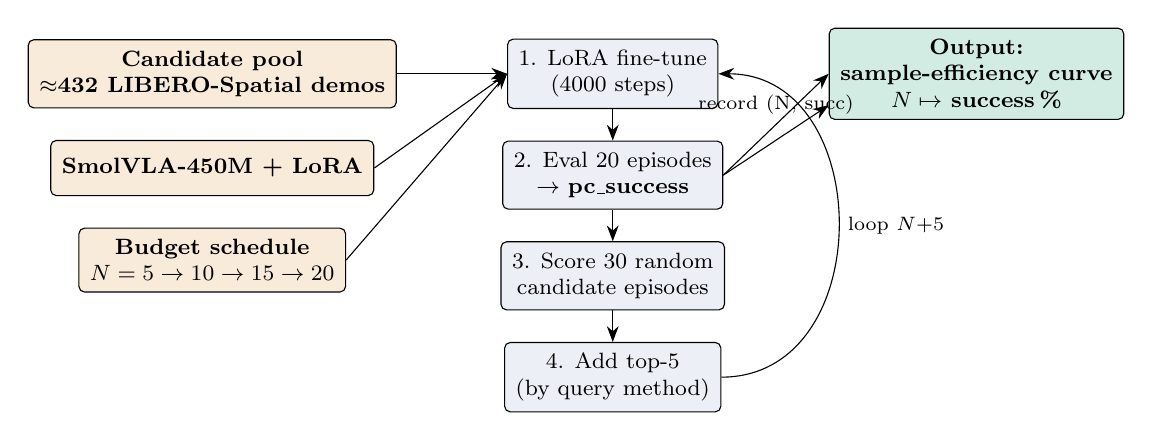
\begin{tikzpicture}[
  font=\footnotesize,
  >={Stealth[length=2mm]},
  node distance=4mm and 6mm,
  box/.style={draw, rounded corners=2pt, align=center, inner sep=4pt, minimum height=7mm, fill=primary!8},
  io/.style={draw, rounded corners=2pt, align=center, inner sep=4pt, minimum height=7mm, fill=accent!15, font=\footnotesize\bfseries},
]
% Inputs
\node[io] (pool) {Candidate pool\\$\approx$432 LIBERO-Spatial demos};
\node[io, below=of pool] (backbone) {SmolVLA-450M + LoRA};
\node[io, below=of backbone] (budget) {Budget schedule\\$N=5\rightarrow 10\rightarrow 15\rightarrow 20$};

% Loop boxes
\node[box, right=14mm of pool] (train) {1. LoRA fine-tune\\(4000 steps)};
\node[box, below=of train] (eval) {2. Eval 20 episodes\\$\to$ \textbf{pc\_success}};
\node[box, below=of eval] (score) {3. Score 30 random\\candidate episodes};
\node[box, below=of score] (add) {4. Add top-5\\(by query method)};

% Output
\node[io, right=14mm of train, fill=good!18] (curve) {Output:\\sample-efficiency curve\\$N \mapsto $ success\,\%};

\draw[->] (pool.east) -- (train.west);
\draw[->] (backbone.east) -- (train.west);
\draw[->] (budget.east) -- (train.west);

\draw[->] (train) -- (eval);
\draw[->] (eval) -- (score);
\draw[->] (score) -- (add);
\draw[->] (add.east) .. controls +(2,0) and +(2,0) .. node[right, font=\scriptsize]{loop $N{+}5$} (train.east);

\draw[->] (eval.east) -- ($(curve.west)+(0,-0.4)$);
\draw[->] (eval.east) -- ($(curve.west)+(0,0.0)$) node[midway, above, font=\scriptsize]{record (N, succ)};
\end{tikzpicture}
\vfill
\muted{\footnotesize 4 rounds per cell. One cell = (method, suite, seed). $\approx$5\,h wall on one RTX\,6000.}
\end{frame}

% --------------------------------------------------------------------
\begin{frame}{Pipeline glossary (what those words mean)}
\footnotesize
\begin{description}
  \setlength{\itemsep}{0.35em}
  \item[Episode] One complete recorded demonstration of a single task attempt \textemdash{} a sequence of (camera images, robot state, action) tuples saved by a human teleop session. LIBERO-Spatial ships $\sim$430 such episodes across 10 tasks (``put X on Y'' variants).

  \item[Candidate pool] All episodes \emph{not yet} in the current training budget. Each round, we pick from this pool.

  \item[Budget schedule \boldmath$N{=}5\to10\to15\to20$] We don't train once at $N{=}20$. We train \emph{four times}: first on 5 demos, then 10, then 15, then 20, adding 5 demos per round. The result is a curve $N \mapsto $ success\,\%. This lets us see \emph{when} the active method beats random, not just whether at one $N$.

  \item[Why subsample 30 random candidates?] Scoring all $\sim$430 candidates needs $\sim$430 SmolVLA forward passes per round (or $4\times$ that for dispersion). Subsampling 30 keeps cost bounded; randomness rotates coverage across rounds.

  \item[Why add top-5 each round?] \texttt{demos\_per\_round=5}. Smaller increments would be invisible eval noise; larger increments would skip past the budgets where active selection matters.

  \item[\texttt{pc\_success}] \emph{Percent-success} on the held-out eval suite: fraction of 20 LIBERO rollouts the trained policy completes, $\times 100$. Range $[0, 100]$. This is the number we plot.
\end{description}
\end{frame}

% --------------------------------------------------------------------
\begin{frame}{Query method 1: \texttt{random}}
\begin{itemize}
  \item \textbf{Input signal}: none.
  \item \textbf{Scoring rule}: score $=$ \texttt{rng.random()} per candidate.
  \item \textbf{Selection rule}: top-5 by score (i.e.\ uniform pick of 5 from 30).
  \item \textbf{Expected failure mode}: bad demos by chance; high seed variance.
  \item \textbf{Why it matters}: the de-facto baseline; if a learner doesn't beat this on a well-pretrained VLA, the acquisition signal is anti-informative.
\end{itemize}
\end{frame}

% --------------------------------------------------------------------
\begin{frame}{Query method 2: \texttt{conformal} \quad\bad{[BROKEN]}}
\begin{itemize}
  \item \textbf{Input signal}: teacher-forced policy loss per candidate episode (12 stride-8 frames, 1 forward pass each).
  \item \textbf{Scoring rule (as implemented)}: per candidate,
    \begin{enumerate}
      \item add its own loss to the calibration buffer,
      \item return \texttt{loss/qhat} if buffer $\geq 20$, else raw \texttt{loss}.
    \end{enumerate}
  \item \textbf{Selection rule}: top-5 by score.
  \item \bad{\textbf{Failure mode (confirmed)}}: self-referential calibration $+$ per-candidate threshold $+$ sorted candidate order $\Rightarrow$ structurally picks \emph{highest-indexed} episodes in the random subsample, not the most uncertain.
  \item See ``Conformal bug'' slide for the full diagnosis.
\end{itemize}
\end{frame}

% --------------------------------------------------------------------
\begin{frame}{Query method 3: \texttt{entropy}}
\begin{itemize}
  \item \textbf{Input signal}: same teacher-forced loss as conformal.
  \item \textbf{Scoring rule}: score $=$ mean loss over sampled frames.
  \item \textbf{Selection rule}: top-5 by score.
  \item \textbf{Expected failure mode}: loss is dominated by nuisance (trajectory length, contact noise, gripper switches), not epistemic uncertainty. Picks redundant ``hard'' demos.
  \item \textbf{Empirical}: trails random by 6-12\,pp at $N{=}20$ (1 seed). Consistent with the nuisance hypothesis.
\end{itemize}
\end{frame}

% --------------------------------------------------------------------
\begin{frame}{Query method 4: \texttt{dispersion}}
\begin{itemize}
  \item \textbf{Input signal}: $K{=}4$ samples from SmolVLA's flow-matching action head per frame; mean per-(step, dim) std across samples.
  \item \textbf{Scoring rule}: score $=$ mean dispersion over sampled frames.
  \item \textbf{Selection rule}: top-5 by score.
  \item \textbf{Why this should help}: measures self-disagreement in \emph{action space}, not next-token likelihood. On a saved checkpoint: dispersion stayed in $[0.037, 0.043]$ while teacher-forced loss spanned $[0.04, 8.69]$ across 4 episodes \textemdash{} loss is mostly nuisance.
  \item \textbf{Failure mode (also confirmed empirically)}: regresses at $N{=}15$ (29\,$\to$\,22\,\%). Without coverage, dispersion overselects from one visually-busy task.
\end{itemize}
\end{frame}

% --------------------------------------------------------------------
\begin{frame}{Query method 5: \texttt{dispersion\_quota}}
\begin{itemize}
  \item \textbf{Input signal}: same as \texttt{dispersion}.
  \item \textbf{Scoring rule}: same as \texttt{dispersion}.
  \item \textbf{Selection rule}: greedy round-robin under per-task coverage. For each pick, choose the candidate from the task with the smallest (budget $+$ already-picked) count; break ties by score.
  \item \textbf{Why this should help}: forces task diversity; prevents the redundant-task collapse that pure dispersion shows.
  \item \textbf{Full N=20 sweep, 4 seeds, paired vs random}: quota wins \good{3 of 4} seeds at the full budget, \good{mean $+9.0$\,pp} (39.4 vs 30.4).
  \item \textbf{Budget interaction}: quota often trails random at $N{=}10/15$ then \good{overtakes at $N{=}20$} (s0, s1, s3 all jump late) \textemdash{} forced task coverage costs early, pays off once the budget covers the suite.
  \item \textbf{Verdict}: diversity-aware action dispersion is \good{robustly} better than random in low-demo SmolVLA/LoRA \textemdash{} not a single-seed fluke. s2 ($-9.5$) is the lone loss, within seed variance.
\end{itemize}
\end{frame}

% --------------------------------------------------------------------
\begin{frame}{Final result: paired N=20, all 4 seeds (libero\_spatial)}
\centering
\begin{tabular}{c|cccc|c}
\toprule
$N{=}20$ & s0 & s1 & s2 & s3 & mean \\
\midrule
random            & 35.0 & 40.5 & 30.0 & 16.0 & 30.4 \\
dispersion\_quota & \good{47.5} & \good{48.0} & \bad{20.5} & \good{41.5} & \good{\textbf{39.4}} \\
\midrule
$\Delta$ & \good{+12.5} & \good{+7.5} & \bad{$-9.5$} & \good{+25.5} & \good{$\mathbf{+9.0}$} \\
\bottomrule
\end{tabular}

\vspace{1.2em}
\begin{itemize}
  \item \textbf{quota wins 3 of 4 seeds at the full budget; mean $+9.0$\,pp.}
  \item Paired demos + paired eval per seed \textemdash{} the gap is not eval noise.
  \item s2 ($-9.5$) is the lone loss; random itself swings $16.0\to40.5$ across seeds, so this is within seed variance.
  \item Earlier conformal/entropy/pure-dispersion all \emph{lost} to random; only \texttt{dispersion\_quota} (dispersion $+$ task coverage) beats it.
\end{itemize}
\end{frame}

% --------------------------------------------------------------------
\begin{frame}{Conformal bug \textemdash{} how scoring went wrong}
\textbf{Codex's invariant check}:\\
if conformal score $=$ \texttt{loss/qhat} with a \emph{global} \texttt{qhat}, ranking $=$ entropy ranking.
\vspace{0.5em}

\textbf{Empirical}: seed-0 $N{=}5{\to}10$ new picks
\begin{itemize}
  \item conformal: $\{1394, 1447, 1458, 1493, 1523\}$
  \item entropy:\hspace{1.05em} $\{1394, 1458, 1567, 1574, 1579\}$
\end{itemize}
Overlap $2/5$. \bad{Invariant violated.}
\vspace{0.5em}

\textbf{Smoking gun in \texttt{active\_loop.py:77\textendash 82}}:
\begin{itemize}
  \item Each candidate's own loss is added to the buffer \emph{before} it is scored (self-reference).
  \item Buffer resets every round; \texttt{calib\_min}$=20$, \texttt{max\_candidates}$=30$.
  \item Candidates $0{-}19$ return raw loss ($\sim$0.03); $20{-}29$ return \texttt{loss/qhat} ($\sim$1.0). 20\,$\times$ scale gap.
  \item Top-5 always lands in the last $\sim$10 iterated candidates $=$ highest-indexed in the sorted subsample.
\end{itemize}
\textbf{Implication}: conformal in this top-$k$ pool setting reduces to a monotone transform; ranking $\equiv$ entropy. The branding adds no acquisition signal.
\end{frame}

% --------------------------------------------------------------------
\begin{frame}{Status \textemdash{} sweep complete}
\textbf{Done}
\begin{itemize}
  \item PS.4 single-task gate passed (80\,\% on libero\_spatial task 0).
  \item 5 methods evaluated; conformal bug found (rank-invariant violated) and documented.
  \item Pure \texttt{dispersion} regresses at $N{=}15$ \good{reproducibly}; conformal \& entropy both lose to random.
  \item \good{Full N=20 sweep complete}: \texttt{dispersion\_quota} beats random on \good{3/4} seeds, mean \good{$+9.0$\,pp}.
\end{itemize}

\textbf{Answered}
\begin{itemize}
  \item Is \texttt{dispersion\_quota} robust, or a one-seed fluke? \good{Robust} \textemdash{} 3/4 at both $N{=}10$ and $N{=}20$, two independent stress tests agree.
\end{itemize}

\textbf{Cost}
\begin{itemize}
  \item GPU contention (HMDB51 co-tenant) stretched the sweep to $\sim$4 days; several cells needed 2\textendash 3 OOM retries. All failures graceful, none lost permanently.
\end{itemize}
\end{frame}

% --------------------------------------------------------------------
\begin{frame}{N=10 stress test (codex-recommended): \good{quota passed}}
\textbf{Design}: fixed $N{=}10$, \texttt{random} vs \texttt{dispersion\_quota}, 4 seeds, paired demos + paired eval. Decision rule set \emph{before} looking at the data.

\vspace{0.6em}
\centering
\begin{tabular}{c|cc|c}
\toprule
seed & random & quota & $\Delta$ \\
\midrule
0 & 22.5 & 25.0 & $+2.5$ \\
1 & 31.0 & 21.5 & \bad{$-9.5$} \\
2 & 28.5 & 36.0 & \good{$+7.5$} \\
3 & 12.5 & 40.0 & \good{$+27.5$} \\
\midrule
mean & 23.6 & \good{30.6} & \good{$\mathbf{+7.0}$} \\
\bottomrule
\end{tabular}

\vspace{0.6em}
\raggedright
\textbf{Verdict}: quota wins \good{3 of 4} seeds; seed 1 is the lone outlier. Rule says: \emph{run full $N{=}20$ curves for quota}. Caveat: $N{=}10$ confirms robustness, not yet the $N{=}20$ magnitude.

\vspace{0.4em}
\muted{\footnotesize Aside: the test cost 8 cells \textemdash{} a recurring co-tenant (HMDB51) OOM-killed the $N{=}10$ rounds 4$\times$; the clean pairs came from running one cell at a time on whichever GPU was momentarily free.}
\end{frame}

% --------------------------------------------------------------------
\begin{frame}{The honest paper, if the method win doesn't hold}
The fallback is \emph{not} a failed project \textemdash{} it is a sharper, more defensible claim:

\vspace{0.6em}
\begin{quote}
\small
For low-demo VLA fine-tuning, acquisition signals that look principled under supervised active learning become \emph{self-referential} (conformal) or \emph{anti-informative} (teacher-forced loss, action dispersion). Under paired demos and paired eval, they fail to robustly beat random; per-task coverage gives single-seed gains that don't generalize. The contribution is a \emph{diagnostic account of why fixed-budget pool AL for VLAs is brittle}, not a new selector.
\end{quote}

\vspace{0.4em}
\textbf{Minimum artifact}: (1) conformal self-reference bug $+$ rank invariant; (2) reproducible $N{=}15$ regression of pure dispersion; (3) random-vs-quota table over $\geq$2 seeds, \emph{labelled as robustness evidence}, not a win.
\end{frame}

\end{document}
